\documentclass{article}
\usepackage[a4paper, total={6in, 8in}]{geometry}
\usepackage{graphicx}
\usepackage{url}
\usepackage{natbib}
\usepackage{todonotes}
\usepackage{booktabs}
\usepackage{lineno}


\linespread{2}

% Title
\title{A Topic Model of Climate Change Literature}
\title{Words, words, words: Mapping the Matter of Climate Change Literature}
\title{A Topography of Climate Change Research}
%\author{Max Callaghan}


\begin{document}
\maketitle

\linenumbers

\textbf{
The massive expansion of scientific literature on climate change challenges the Intergovenmental Panel on Climate Change (IPCC)'s ability to assess the science according to its objectives. 
Moreover, the number and variety of papers hinders researchers of the science-policy interface from making objective judgements about those IPCC's assessments. In this paper, we present a novel application of a machine-reading approach to model the topical content of papers on climate change. This dynamic topic model provides the basis for a \textit{topography} of climate change literature. The thematic development of the field is outlined and used to inform an analysis of the topics which are better and less well covered by IPCC reports.
}


The IPCC sees its role as to ``assess on a comprehensive, objective, open and transparent basis the scientific, technical and socio-economic information relevant to [...] climate change'' \citep{IPCC2013}. This role is vital....

Various researchers have attempted to analyse the IPCC's assessment reports, criticised the assessment processes of the IPCC. ref ref ref. Further, it has been pointed out that, in the age of ``big literature'', providing assessments that are comprehensivene, objective and transparent has become much more difficult \citep{Minx2017l}. 

The scale of the challenge is depicted in figure \ref{growth}. Less than two thousand documents relevant to climate change were published before the first assessment report (see Methods for data, exclusions and processing). These documents contained 3,528 unique terms, each of which was used on average in 0.49\% of documents. In the three complete years since the publication of AR5, 128,357 documents have been published, containing 86,419 unique terms. To put this into context, the 1,189 chapters of the Bible contain a vocabulary of 11,977 unique words. Put another way, the 236,634 publications published in AR5 and AR6 are significantly larger than the 178,118 publications recorded in the first volume of the `Catalogue of Scientific Papers', compiled by the Royal Society to record the entirety of scientific output from 1800 to 1863 \citep{Csiszar2017}

\begin{figure}
	\begin{center}
		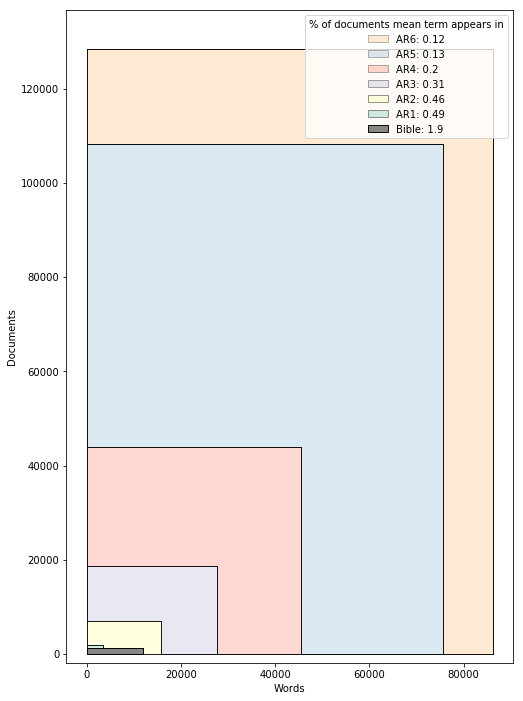
\includegraphics[width=0.7\linewidth]{plots/volume_variety}
		\caption{The volume and variety of literature on climate change has grown to unmanageable proportions. Each box represents a document-term matrix (unique documents x unique terms) of the abstracts written in each assessment period. The proportion of documents the average word occurs in is given in the key.
		}
		\label{growth}
	\end{center}
\end{figure}
	

Clearly, if the IPCC is to continue producing comprehensive assessments, it has to engage in machine-reading in order to remain anchored to the wider literature. Without such an approach, it becomes harder to justify which ever-diminishing proportion of the wider literature is included in assessments. Indeed this same approach is required if researchers are to make convincing claims about what areas of the literature are well-covered, and what are overlooked.

This paper uses 


\section*{Results}


\begin{figure}
\begin{center}
	%\includegraphics[width=0.7\linewidth]{}
    \caption{}
    \label{}
    \end{center}
\end{figure}


\section*{Methods}
\label{methods}

\listoffigures
\linespread{1}
\bibliography{Mendeley.bib}
\bibliographystyle{unsrt}

\end{document}

